\documentclass{scrartcl}
\usepackage[utf8]{inputenc}
\usepackage{graphicx}
\usepackage{wrapfig}
\usepackage{listings}
\usepackage{minted}
\usepackage{subcaption}
\usepackage{csquotes}
\usepackage{hyperref}
\usepackage{amsmath}


\title{PLSC 504: Replication Term Paper}
\subtitle{Secular Party Rule and Religious Violence in Pakistan}
\author{Mario Belledonne}
\date{\today}

\begin{document}

\maketitle

\section{Introduction}


\section{Theory}

Do terrorists cause violence in response to secular incumbency or does secular incumbency occur in response to terrorist violence?

The period of $1998 \rightarrow 2003$ in Pakistan offers a "natural experiment" due to a plurality of first-past-the-post elections where both Islamist and secular leaders compete. 
These elections determine the Members of the National Assembly (MNA). The MNA are responsible for implementing local policies at the behest of their constituency and have also been known to collaborate with other local officials, notably police, in order to fulfill these goals. 

The authors claim that the proportion of secular victories within a MNA district can influence violence directly (via policy) or indirectly by interactions with local officials (the police). 

For both mechanisms, the authors claim that provincial and temporal fixed effects may be present. These are described in more detail in \ref{identification}.

\ref{figure:id-dag} illustrates the causal model used in the following sections.

\section{Design}

\subsection{Identification} \label{identification}

\subsubsection{The Outcome Variable}

The authors used reports from the BFRS Political Violence in Pakistan Dataset. This dataset tallied reports of political violence from a daily English-language newspaper, \textit{Dawn}. The geo-political units of these reports are in terms of administrative districts. This immediately posses a challenge to identification since administrative units do not correspond in a one-to-one fashion to constituencies and have re-organized over time.

The authors define a novel geo-political unit of analysis to overcome the discrepancy between districts and constituencies: the \textit{joined-district}. 
This is defined as:
\begin{displayquote}
...the smallest amalgamation of districts that encompasses complete MNA constituencies. 
\end{displayquote}

The $Y_{i,t}$ thus describes the level of religious violence for a particular joined-district $i$ at election year $t$. The authors use a variety of outcomes for religious violence described below. 

\begin{enumerate}
\item Any Event: A binary variable that is \textit{True} if any form of religious violence occured during the MNA's time in office for that district
\item Any Killed: Similar to \textit{Any Event} but referring to any deaths
\item Event Count: The number of religious-violent events
\item Number Killed: The number of deaths caused by religious violence
\item Number of days: The number of days in which at least one instance of religious violence occured.
\end{enumerate}

To capture the time varying nature of administrative districts (and thus the relevance the joint-district unit), the authors included a second unit, the \textit{cluster district} that is define as follows:

\begin{displayquote}
  the smallest amalgamation of districts that contain complete MNA constituencies that did not geographically change from $1998 - 2013$.
\end{displayquote}

These cluster districts where used in calculating clustered standard errors.

\subsubsection{Treatment}

The authors define treatment as

\begin{displayquote}
... the proportion of joined-district MNA seats
  won by secular party candidates ...
\end{displayquote}


\subsubsection{Covariates}

\subsection{Fuzzy RD as IV}

\begin{equation} \label{eq:1}
  Y_{i,t} = \alpha + \beta * D_{i,t} + \epsilon_{i,t}
\end{equation}

Where, $D_{i,t}$ is the treatment and $\epsilon_{i,t}$ describes error.\\

The authors note in \ref{eq:1} that there may be an issue of reverse causality with this estimator. Namely, that violence in a previous period could effect the outcome and treatment for the subsequent period.
To this effect, the authors claim to define period of exogenous variation within close elections between secular and Islamist candidates.

Thus they define a two stage estimation strategy as follows:


\begin{equation} \label{eq:2}
  \widehat{D_{i,t}} = \mu + \lambda * Z_{i,t} + \kappa*D_{i,t} + \theta_p + v_{i,t}
\end{equation}

\begin{equation} \label{eq:3}
  Y_{i,t} = \alpha + \beta * \widehat{D_{i,t}} + \gamma*D_{i,t} + \theta_{p} + \epsilon_{i,t}
\end{equation}

Where

\begin{itemize}
\item $Z_{i,t}$ describes the proportion of MNA seats won by secular candidates when in close competition with Islamist candidates (within $\pm 3\%$).
\item $\widehat{D_{i,t}}$ is the predicted proportion of MNA seats won by secular candidates across all races in that district.
\item $\theta_p$ describes a geo-spatial fixed effect of violence reporting at the province level. 
\end{itemize}

Here \ref{eq:2} refers to the first stage and \ref{eq:3} refers to the estimator of the \texttt{ATE} localized to close races between secular and Islamist MNA elections.  

\begin{figure}[h]
  \centering
  \scalebox{0.5}{
    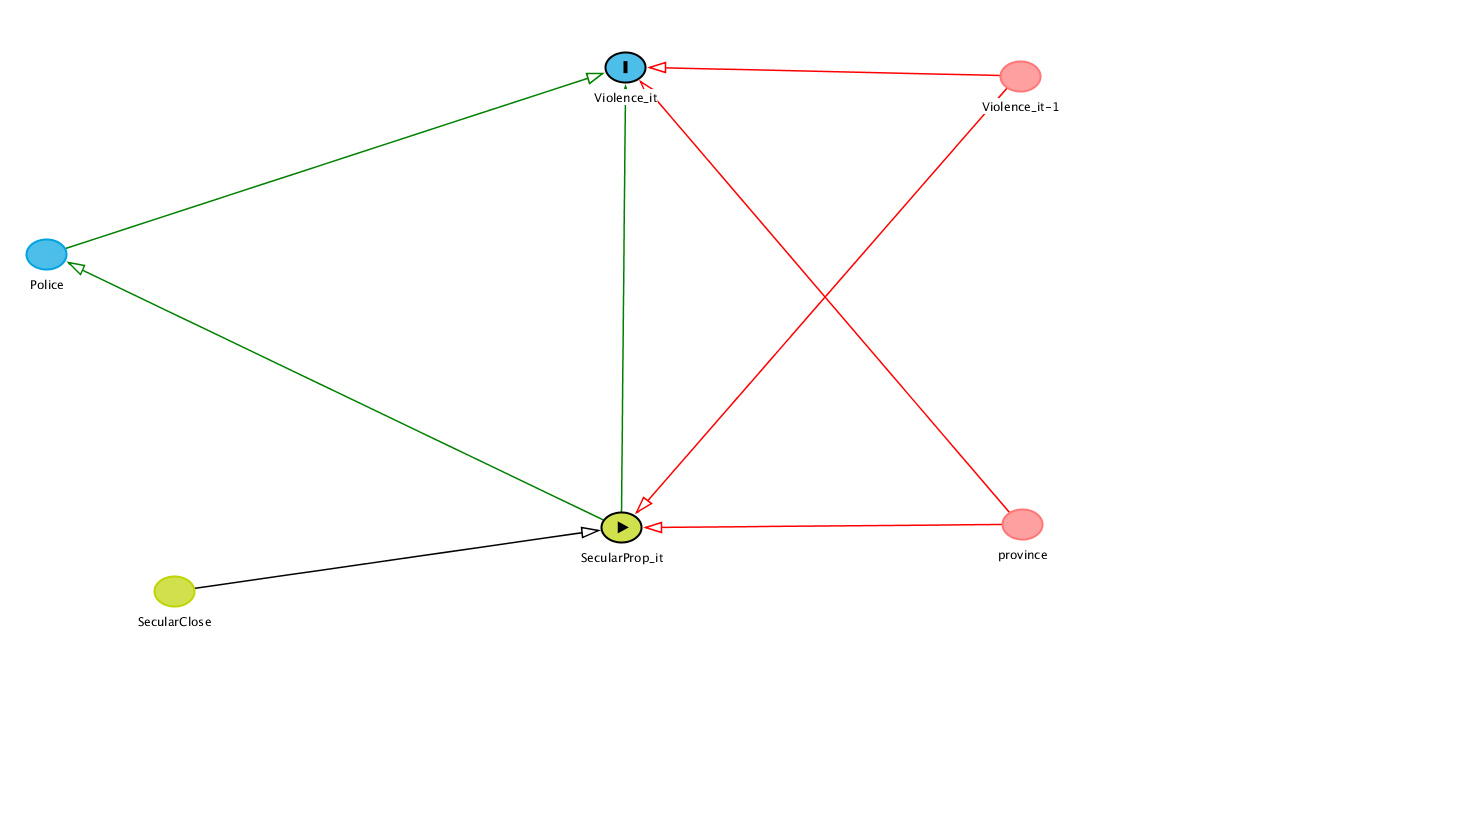
\includegraphics{replication/dag.png}
  }
  \caption{DAG for Fuzzy RD Identification}
  \label{fig:iv-dag}
\end{figure}

In sum the authors' assumptions are described in Fig \ref{fig:iv-dag}

\section{Results}

\subsection{Main Effect}

\subsubsection{IV Estimates of Main Effect}

\begin{table}[ht]
  \begin{center}
    \scalebox{0.75}{
      
\begin{table}
\begin{center}
\begin{tabular}{l c c c c c }
\hline
 & Any Event & Event Count & Any Killed & Number Killed & Number Days \\
\hline
Prop. Secular Win        & $-0.660^{*}$        & $-4.654^{*}$        & $-0.477$           & $-3.266$           & $-4.700^{*}$        \\
                         & $[-1.152;\ -0.168]$ & $[-8.658;\ -0.649]$ & $[-1.112;\ 0.159]$ & $[-8.222;\ 1.689]$ & $[-8.760;\ -0.640]$ \\
Prop. Secular Clost Race & $0.031$             & $0.837$             & $0.004$            & $0.281$            & $0.947$             \\
                         & $[-0.166;\ 0.227]$  & $[-1.223;\ 2.897]$  & $[-0.389;\ 0.396]$ & $[-2.814;\ 3.376]$ & $[-1.135;\ 3.029]$  \\
\hline
R$^2$                    & -0.580              & -0.486              & -0.164             & -0.169             & -0.482              \\
Adj. R$^2$               & -0.602              & -0.507              & -0.180             & -0.185             & -0.503              \\
Num. obs.                & 437                 & 437                 & 437                & 437                & 437                 \\
RMSE                     & 0.357               & 3.025               & 0.389              & 3.194              & 3.114               \\
\hline
\multicolumn{6}{l}{\scriptsize{Robust SEs clustered by cluster-district area, in brackets}}
\end{tabular}
\caption{TABLE 2. Instrumental Variable Results}
\label{table:coefficients}
\end{center}
\end{table}

    }
    \caption{Instrumental Variable Results}
    \label{table:2}
  \end{center}
\end{table}

I was able to reproduce the estimated \texttt{ATE} with discrepancies in the standard errors using the \texttt{estimatr::iv\_robust} method in \texttt{R}.
That being said, the negative effect of proportion of secular victories on whether a joined-district had any event of religious violence and the number of religious violent events survived this replication table \ref{table:2}.

A potential explanation for the difference in SEs could be do to the authors not using robust standard error calculation. (will look into this more).


\subsection{Difference in Means}

\begin{table}[ht]
  \begin{center}
    \scalebox{0.75}{
      
\begin{table}
\begin{center}
\begin{tabular}{l c c c c c }
\hline
 & Any Event & Event Count & Any Killed & Number Killed & Number Days \\
\hline
Secularist Close Win & $-0.176$           & $-1.265$           & $-0.141$           & $-0.769$           & $-1.265$           \\
                     & $[-0.373;\ 0.020]$ & $[-2.654;\ 0.123]$ & $[-0.331;\ 0.049]$ & $[-2.142;\ 0.605]$ & $[-2.654;\ 0.123]$ \\
\hline
R$^2$                & 0.330              & 0.393              & 0.398              & 0.390              & 0.393              \\
Adj. R$^2$           & 0.267              & 0.336              & 0.341              & 0.332              & 0.336              \\
Num. obs.            & 59                 & 59                 & 59                 & 59                 & 59                 \\
RMSE                 & 0.279              & 2.303              & 0.280              & 2.435              & 2.304              \\
\hline
\multicolumn{6}{l}{\scriptsize{Robust SEs clustered by cluster-district area, in brackets}}
\end{tabular}
\caption{TABLE 3. Instrumental Variable Results}
\label{table:coefficients}
\end{center}
\end{table}

    }
    \caption{Difference in Means Estimate}
    \label{table:3}
  \end{center}
\end{table}

In an effort to appeal to the strength of their data and design, the authors attempt to estimate the \texttt{ATE} using the difference-in-means estimator (table \ref{table:3}).
To this end, the authors restrict the dataset to 59 years and joined-district points where there was a single close election between secular and Islamist candidates.

Again, the estimated effects match the original but due to a difference in SEs, none of the estimates survived replication. In the original, the authors report a significant effect for \textit{Any Event, Event Count, Number days}.

%% \begin{center}
%% \footnotesize 
\begin{table}
\begin{center}
\begin{tabular}{l c c c c c }
\hline
 & Any Event & Event Count & Any Killed & Number Killed & Number Days \\
\hline
Secularist Close Win & $-0.176$           & $-1.265$           & $-0.141$           & $-0.769$           & $-1.265$           \\
                     & $[-0.373;\ 0.020]$ & $[-2.654;\ 0.123]$ & $[-0.331;\ 0.049]$ & $[-2.142;\ 0.605]$ & $[-2.654;\ 0.123]$ \\
\hline
R$^2$                & 0.330              & 0.393              & 0.398              & 0.390              & 0.393              \\
Adj. R$^2$           & 0.267              & 0.336              & 0.341              & 0.332              & 0.336              \\
Num. obs.            & 59                 & 59                 & 59                 & 59                 & 59                 \\
RMSE                 & 0.279              & 2.303              & 0.280              & 2.435              & 2.304              \\
\hline
\multicolumn{6}{l}{\scriptsize{Robust SEs clustered by cluster-district area, in brackets}}
\end{tabular}
\caption{TABLE 3. Instrumental Variable Results}
\label{table:coefficients}
\end{center}
\end{table}

%% \end{center}{}
%% \begin{center}
%% \footnotesize 
\begin{table}
\begin{center}
\begin{tabular}{l c c c }
\hline
 & No Fixed Effects & Disctrict Cluster FE & Disctrict Cluster + Province-Year FEs \\
\hline
Secularist Close Race & $-0.355^{*}$        & $-0.386^{*}$        & $-0.257^{*}$        \\
                      & $[-0.613;\ -0.096]$ & $[-0.613;\ -0.159]$ & $[-0.441;\ -0.073]$ \\
\hline
R$^2$                 & 0.027               & 0.294               & 0.497               \\
Adj. R$^2$            & 0.025               & 0.194               & 0.386               \\
Num. obs.             & 437                 & 437                 & 437                 \\
RMSE                  & 0.371               & 0.337               & 0.294               \\
\hline
\multicolumn{4}{l}{\scriptsize{Robust SEs clustered by cluster-district area, in brackets}}
\end{tabular}
\caption{TABLE 4. Correlation Between Close Secular/Nonsecular Elections and Violence at Time t-1}
\label{table4}
\end{center}
\end{table}

%% \end{center}{}
\subsection{Robustness and Balance Checks}

\subsubsection{Reverse Causality for Treatment and Instrument}

\begin{table}[ht]
  \begin{center}
    \scalebox{0.75}{
      
\begin{table}
\begin{center}
\scalebox{0.5}{
\begin{tabular}{l c c c c c }
\hline
 & Any Event & Event Count & Any Killed & Number Killed & Number Days \\
\hline
Prop. Secular Win        & $-0.066$           & $-1.165$           & $-0.127$           & $-1.404$           & $-1.162$           \\
                         & $[-0.643;\ 0.511]$ & $[-5.624;\ 3.295]$ & $[-0.686;\ 0.433]$ & $[-5.889;\ 3.080]$ & $[-5.621;\ 3.298]$ \\
Prop. Secular Clost Race & $-0.364$           & $-1.802$           & $-0.313$           & $-1.696$           & $-1.811$           \\
                         & $[-0.755;\ 0.027]$ & $[-4.997;\ 1.393]$ & $[-0.715;\ 0.089]$ & $[-5.031;\ 1.638]$ & $[-5.005;\ 1.383]$ \\
\hline
R$^2$                    & 0.137              & 0.129              & 0.117              & 0.091              & 0.129              \\
Adj. R$^2$               & 0.125              & 0.117              & 0.105              & 0.078              & 0.116              \\
Num. obs.                & 437                & 437                & 437                & 437                & 437                \\
RMSE                     & 0.301              & 2.535              & 0.355              & 2.904              & 2.540              \\
\hline
\multicolumn{6}{l}{\scriptsize{Robust SEs clustered by cluster-district area, in brackets}}
\end{tabular}
}
\caption{Placebo Check — Can Secular Victory in Close Elections at Time t Predict Prior Violence}
\label{table1}
\end{center}
\end{table}

    }
    \caption{Placebo Check — Can Secular Victory in Close Elections at Time t Predict Prior Violence}
    \label{table:1}
  \end{center}
\end{table}

In order to address the potential influence of reverse causality, the authors attempted to predict the previous outcome for a given joined-district $Y_{i,t-1}$.
I was able to reproduce the authors' null result \ref{table:1}.

\begin{table}[ht]
  \begin{center}
    \scalebox{0.75}{
      
\begin{table}
\begin{center}
\begin{tabular}{l c c c }
\hline
 & No Fixed Effects & Disctrict Cluster FE & Disctrict Cluster + Province-Year FEs \\
\hline
Secularist Close Race & $-0.355^{*}$        & $-0.386^{*}$        & $-0.257^{*}$        \\
                      & $[-0.613;\ -0.096]$ & $[-0.613;\ -0.159]$ & $[-0.441;\ -0.073]$ \\
\hline
R$^2$                 & 0.027               & 0.294               & 0.497               \\
Adj. R$^2$            & 0.025               & 0.194               & 0.386               \\
Num. obs.             & 437                 & 437                 & 437                 \\
RMSE                  & 0.371               & 0.337               & 0.294               \\
\hline
\multicolumn{4}{l}{\scriptsize{Robust SEs clustered by cluster-district area, in brackets}}
\end{tabular}
\caption{TABLE 4. Correlation Between Close Secular/Nonsecular Elections and Violence at Time t-1}
\label{table4}
\end{center}
\end{table}

    }
    \caption{Correlation Between Close Secular/Nonsecular Elections and Violence at Time t-1}
    \label{table:4}
  \end{center}
\end{table}

The authors also computed the predictive capacity of the instrument for lagged violence.
These results are reported in table \ref{table:4} which replicate the source.
Both with and without time and provincial fixed effects, the instrument is able to predict a lower level of religious violence.

The authors claim that this limits the external validity of their main effect. I would argue that this also damages the internal validity as the instrument is shown to be likely endogenous and this the IV 2SLS estimate is likely to be biased. 


\subsection{Mechanisms}

The later section of the source, the authors perform explanatory analysis to illustrate potential mechanisms of secular MNA seats on religious violence. One explored avenue was the electoral accountability. The authors claim that secular leaders often include diminished religious violence as a campaign promise. The authors then predict that secular MNA candidates expect to suffer in future elections if religious violence does occur during their tenure. 

To test their prediction, the authors estimate the causal effect of religious violence in the previous term on the proportion of secular MNA seats in the following election.
I was able to reproduce these estimates in full (table \ref{table:5})

\begin{table}[ht]
  \begin{center}
    \scalebox{0.75}{
      
\begin{tabular}{l c c c c }
\hline
 &  &  &  &  \\
\hline
Prop. Secular (t-1) x Any violence     & $-0.115^{*}$        &                     & $-0.102^{*}$        &                     \\
                                       & $[-0.191;\ -0.038]$ &                     & $[-0.185;\ -0.019]$ &                     \\
Prop. Secular (t-1) x Event count (ln) &                     & $-0.018^{*}$        &                     & $-0.014^{*}$        \\
                                       &                     & $[-0.030;\ -0.005]$ &                     & $[-0.028;\ -0.000]$ \\
Any violence                           & $0.105^{*}$         &                     & $0.086^{*}$         &                     \\
                                       & $[0.052;\ 0.157]$   &                     & $[0.039;\ 0.132]$   &                     \\
Prop. secularist wins (t - 1)          & $0.038$             & $-0.053^{*}$        & $0.050$             & $-0.030$            \\
                                       & $[-0.046;\ 0.122]$  & $[-0.101;\ -0.004]$ & $[-0.047;\ 0.146]$  & $[-0.090;\ 0.030]$  \\
Event count                            &                     & $0.018^{*}$         &                     & $0.015^{*}$         \\
                                       &                     & $[0.010;\ 0.026]$   &                     & $[0.006;\ 0.023]$   \\
\hline
R$^2$                                  & 0.656               & 0.657               & 0.734               & 0.733               \\
Adj. R$^2$                             & 0.589               & 0.590               & 0.659               & 0.657               \\
Num. obs.                              & 344                 & 344                 & 344                 & 344                 \\
RMSE                                   & 0.139               & 0.138               & 0.126               & 0.127               \\
\hline
\multicolumn{5}{l}{\scriptsize{Robust SEs clustered by cluster-district area, in brackets}}
\end{tabular}

    }
    \caption{Mechanisms - Electoral Incentives}
    \label{table:5}
  \end{center}
\end{table}


\section{Future work}

\subsection{Robustness Checks of Main Effect}

The authors conduct extensive checks on the implications of their design, including first stage (shown to be weak) and bandwidth sensitivity. 

Issues with the weak instrumental variable non-withstanding, I plan to revisit their bandwidth sensitivity analysis using the \texttt{rdrobust} package to verify that their main effect still holds under MSE-optimal bandwidths.

In addition, the authors investigate the specificity of the effect of secular victories on religious violence to see if secular victories reduce violence in general. 

\subsection{Mechanisms of Main Effect}

The authors illustrate potential mechanisms for their main finding (the reduction of religious violence due to secular victories). These include electoral incentives (in terms of voter accountability if religious violence does arise in the presence of a secular district), politician characteristics, state capacity (concentration of police force in secular districts).

\section{Conclusion}

\bibliography{main}
\bibliographystyle{plain}

\end{document}
